\documentclass{beamer}
\usepackage{colortbl}
\usepackage{graphicx}
\usepackage{ulem}

\usepackage{amsmath}
\usepackage{amssymb}
\usepackage{color}

\renewcommand{\familydefault}{\sfdefault}

% syntactic coloring
% by default, beamer-colors are
%    normal text is black on white.
%    alerted text is red.
%    example text is a dark green (green with 50% black).
%    structure is set to a light version of MidnightBlue (more precisely, 20% red, 20% green, and 70% blue).

\setbeamercolor{key point}{parent=alerted text}

\def\struct{\usebeamercolor[fg]{structure}}
\def\key{\em \usebeamercolor[fg]{key point}}
\def\aside{\scriptsize \usebeamercolor[fg]{example text}}
\def\newthing{\usebeamercolor[fg]{key point}}
\def\oldthing{\usebeamercolor[fg]{structure}}
\def\defthing{\usebeamercolor[fg]{structure}}

% \definecolor{blue}{rgb}{0.05,0.6,1}
% \definecolor{orange}{rgb}{1,0.549,0}
% \definecolor{dark-red}{rgb}{.4,.1,.1}
% \definecolor{pink}{rgb}{1,.8,.8}
% \definecolor{dark-green}{rgb}{.1,.6,.1}
% \definecolor{light-green}{rgb}{.8,1,.8}
% \definecolor{blue-white}{rgb}{.95,.95,1}
% \definecolor{purple}{rgb}{1, 0.0, 0.6}

\newcommand{\R}{\mathbb{R}}
\newcommand{\Q}{\mathbb{Q}}
\newcommand{\Z}{\mathbb{Z}}
\newcommand{\N}{\mathbb{N}}
\newcommand{\C}{\mathbb{C}}

\renewcommand{\P}{\mathbb{P}}
\newcommand{\E}{\mathbb{E}}

\newcommand{\var}{\mathop{\mbox{Var}}}
\newcommand{\cov}{\mathop{\mbox{cov}}}
\newcommand{\median}{\mathop{\mbox{median}}}
%\newcommand{\det}{\mathop{\mbox{det}}}
\newcommand{\supp}{\mathop{\mbox{supp}}}
\newcommand{\sgn}{\mathop{\mbox{sgn}}}

\newcommand{\conv}{\mathop{\mbox{conv}}}
\newcommand{\deq}{\stackrel{\scriptscriptstyle{d}}{=}}
\newcommand{\dcv}{\stackrel{\scriptscriptstyle{d}}{\longrightarrow}}


\newcommand{\figcredit}[1]{{\begin{flushright}\usebeamercolor[fg]{structure} \it \tiny #1 \end{flushright}}}
\newcommand{\fullslide}[1]{\makebox[\linewidth]{\parbox{1.2\textwidth}{#1}}}


\newcommand{\basedir}{files}

%%% macros
\def\migrate{\lambda_{\text{mig}}}
\def\mutrate{\lambda_{\text{mut}}}
\def\Tmig{T_{\text{mig}}}
\def\Tmut{T_{\text{mut}}}
\newcommand\mapsfrom{\mathrel{\reflectbox{\ensuremath{\mapsto}}}}

\setbeamertemplate{blocks}[default]
\usecolortheme{rose}

\mode<presentation>
{
  % \usetheme{default}
  \usetheme{boxes}
  % or ...
  \usefonttheme[options]{structuresmallcapsserif}

  \setbeamercovered{transparent}
  % or whatever (possibly just delete it)
}


\usepackage[english]{babel}
% or whatever

\usepackage[latin1]{inputenc}
% or whatever

\usepackage{times}
\usepackage[T1]{fontenc}
% Or whatever. Note that the encoding and the font should match. If T1
% does not look nice, try deleting the line with the fontenc.


\title % (optional, use only with long paper titles)
{ Population Genomics \\ 
of the Mojave Desert Tortoise  }

\author % (optional, use only with lots of authors)
{Peter Ralph}
% - Use the \inst{?} command only if the authors have different
%   affiliation.

\institute[UO]
{
    University of Oregon \\ Biology \& Mathematics
}
% - Use the \inst command only if there are several affiliations.
% - Keep it simple, no one is interested in your street address.

\date % (optional)
{Evolution! \\ Austin, June 18, 2016}

\def\Put(#1,#2)#3{\leavevmode\makebox(0,0){\put(#1,#2){#3}}}


\begin{document}

\begin{frame}
  \titlepage
\end{frame}

\begin{frame}{the Mojave Desert Tortoise: \only<1>{ \it Gopherus agassizii}}
    \begin{center}
  \includegraphics<1>[width=\textwidth]{\basedir/tortoise-in-burrow}
  \includegraphics<2>[width=.9\textwidth]{\basedir/range-abundance-map}
  \includegraphics<3>[height=.8\textheight]{\basedir/ivanpah-opens}
  \includegraphics<4>[height=.8\textheight]{\basedir/latimes-torts-delay-solar}
    \end{center}
\end{frame}

%%%%%%%%
\begin{frame}{The question(s)}
  \begin{columns}[c]
    \begin{column}{.4\textwidth}

        {\Large How will changes to the landscape affect population viability and gene flow?}

        \vspace{3em}

        {\newthing \large How do tortoises move around on the landscape?}


    \end{column}
    \begin{column}{.6\textwidth}
      \begin{center}

        \vfill
        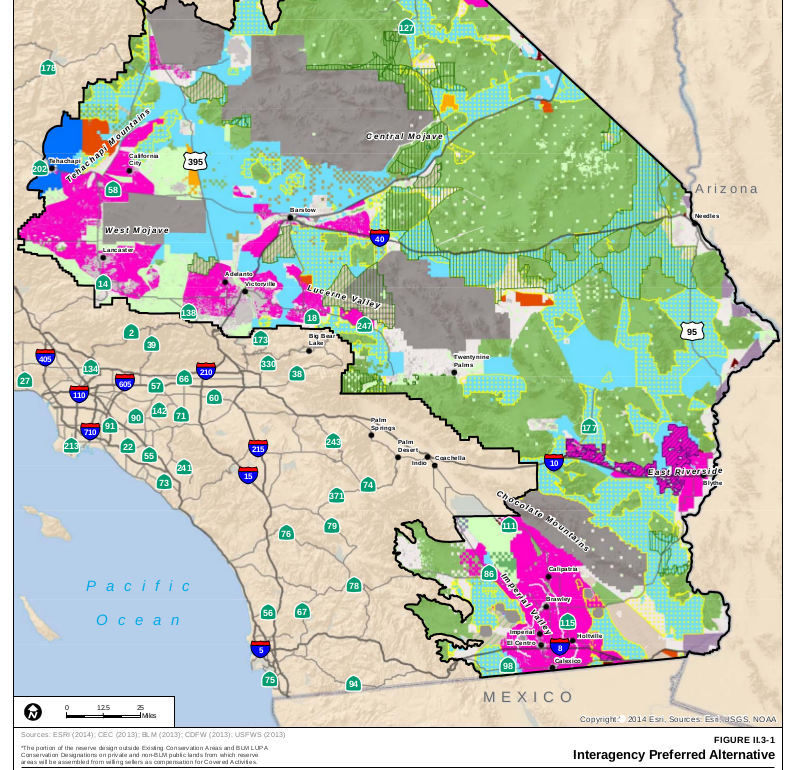
\includegraphics[width=\textwidth]{\basedir/drecp-pref-alt-snapshot}
        \vfill

          % % \vspace{-4em}
          % \includegraphics[width=.7\textwidth]{\basedir/hagerty-2011-habitat-model}
          % \figcaption{Habitat predicted by 12-variable model, with least-cost paths,
          %     from 20 microsats.
           {\aside (Hagerty, Nussear, Esque, \& Tracy 2011)}

      \end{center}
    \end{column}
  \end{columns}
\end{frame}


%%%%%%%%
\begin{frame}{Data}
  \begin{columns}
    \begin{column}{.5\textwidth}

      Thanks to
      {\newthing \bf lots of hard work},
      we have
      \begin{itemize}
          \item<1-> 83 GIS layers at 30m -- {\newthing \it Jannet Vu (UCLA)}
          \item<2-> tissue samples 
              -- {\newthing \it Dick Tracy, Chava Weitzman (UNR), Fran Sandmeier (U.\ Lindenwood), Bridgette Hagerty (York)} \\
              \uncover<3->{\oldthing \large What's in a tortoise nose? 10am Tue}
          \item<4-> 270 tortoises chosen for sequencing -- {\newthing \it Evan McCartney-Melstad (UCLA)}
            %: whole-genome sequences, average {\newthing 1.5x coverage}, ${}>10^{12}$ bp -- Evan McCartney-Melstad (UCLA)
          % \begin{itemize}
          %   \item<4-> mapped to Galapagos Tortoise
          % \end{itemize}
      \end{itemize}

    \end{column}
    \begin{column}{.5\textwidth}
      \begin{center}

          \includegraphics<1>[width=\textwidth]{\basedir/raster-list}
          \includegraphics<2-3>[width=\textwidth]{\basedir/fieldwork}
          \includegraphics<4>[height=.8\textheight]{\basedir/sample_map_elev}
          % \includegraphics<4>[width=\textwidth]{\basedir/tortCoverages-cropped}

      \end{center}
    \end{column}
  \end{columns}
\end{frame}

\begin{frame}{Sequencing \& Bioinformatics}

    {\newthing \it Evan McCartney-Melstad (UCLA)}

    \begin{itemize}
        \item PCR-free library preparation
        \item Illumina 100bp PE: ${}>10^{12}$ bp
        \item read QC, trimming, and joining
        \item map to draft genome 
            (1.9 Gb, Kusumi et al, in prep) \\
            $\approx 1.5\times$ coverage
        \item identify polymorphic sites with \texttt{angsd}  \\
            ($\approx 3\%$ with $p<10^{-6}$)
        \item read-based estimation of divergence \\
            (using $Q\ge30$ bases)
    \end{itemize}

\end{frame}


\begin{frame}{Mitochondria}

    \begin{itemize}
        \item median coverage: $25 \times$
        % \item NuMts -- regions with consistent ``heterozygosity''
        \item % excluding these, 
            per-base error rate of $(2.22 \pm 0.12)\times 10^{-4}$ 
        \item<2-> two haplotypes differing by 0.3\%
    \end{itemize}
  \begin{overlayarea}{\textwidth}{0.5\textheight}
      \centering
    % \includegraphics<1>[width=\textwidth]{\basedir/minor-freq-along-mt}
    % \includegraphics<1>[height=0.55\textheight]{\basedir/error_estimates}
    \includegraphics<2>[height=0.55\textheight]{\basedir/mt-hap-map}
  \end{overlayarea}

\end{frame}

%%%%%%%%
\begin{frame}{Autosomes: PCA}
    \centering
    
    PCA from covariance matrix of {\newthing raw allele counts}

    \hfill
    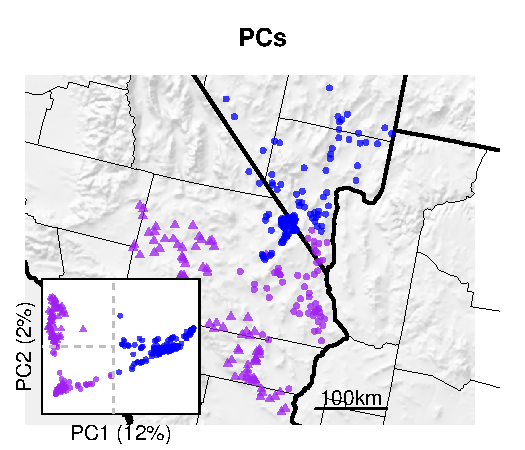
\includegraphics[width=0.54\textwidth]{\basedir/continuous_pc_colors_sample_map}
    \hfill
    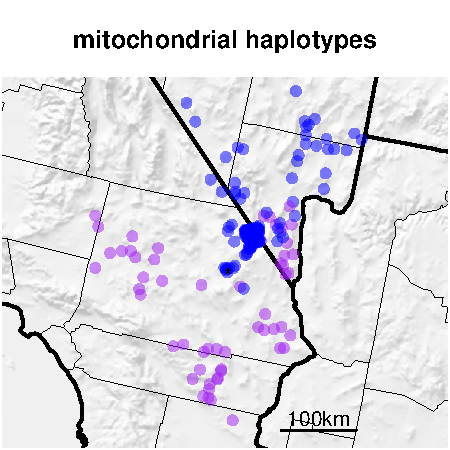
\includegraphics[width=0.46\textwidth]{\basedir/mt-hap-map}
    \hfill
\end{frame}

% %%%%%%%%
% \begin{frame}{Clinal contigs?}
%     \centering
% 
%     A few contigs show strong correlation with PC1:
% 
%     XXX
% 
% \end{frame}

%%%%%%%%
\begin{frame}{Sequence divergence: autosomes}
  \centering
        % made in tortoisescape/visualization/talk-plots.R
        \includegraphics<1>[width=\textwidth]{\basedir/everyone-pwp-shaded}
        \includegraphics<2>[width=\textwidth]{\basedir/pwp_etort-191_shaded}
        \includegraphics<3>[width=\textwidth]{\basedir/pwp_etort-57_shaded}
        \includegraphics<4>[width=\textwidth]{\basedir/pwp_etort-71_shaded}
        \includegraphics<5>[width=\textwidth]{\basedir/pwp_etort-35_shaded}
        \includegraphics<6>[width=\textwidth]{\basedir/pwp_etort-285_shaded}
        \includegraphics<7>[width=\textwidth]{\basedir/pwp_etort-78_shaded}
        \includegraphics<8>[width=\textwidth]{\basedir/pwp_etort-229_shaded}
        \includegraphics<9>[width=\textwidth]{\basedir/pwp_etort-27_shaded}
        \includegraphics<10>[width=\textwidth]{\basedir/pwp_etort-273_shaded}
        \includegraphics<11>[width=\textwidth]{\basedir/pwp_etort-253_shaded}
        \includegraphics<12>[width=\textwidth]{\basedir/pwp_etort-240_shaded}
        \includegraphics<13>[width=\textwidth]{\basedir/pwp_etort-283_shaded}

    \begin{align*}
        \text{divergence} &= \text{(mean density of nucelotide differences)} \approx 0.5\% \\
            &= 2 \text{(years)} \times \text{( mutation rate )}
    \end{align*}

    \vspace{1em} 

    {\aside divergence $\times$ calibrated to painted turtle}

\end{frame}


%%%%%%%
\begin{frame}{Following a lineage}
  \begin{columns}
    \begin{column}{.5\textwidth}
      \centering
      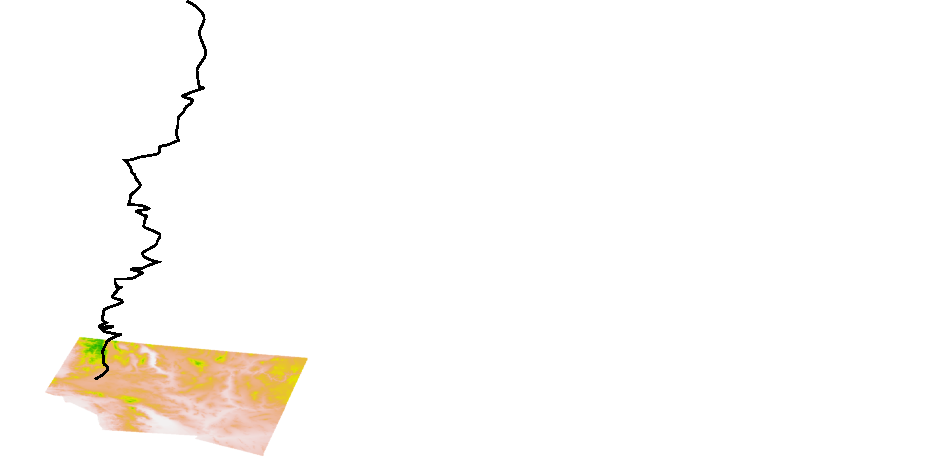
\includegraphics{\basedir/lineages-hitting-time-onelineage}
    \end{column}
    \begin{column}{.5\textwidth}
      A {\newthing single lineage} back through time: \\
      \begin{itemize}
          \item jump rate is mean age of parent at birth
          \item tends to move towards regions that produce more offspring
      \end{itemize}


    \end{column}
  \end{columns}
\end{frame}

%%%%%%%
\begin{frame}{Model for lineage movement}

  Recall that we have {\newthing landscape variables}, e.g.,
  \begin{align*}
    g_1(x) &= ( \text{ elevation at $x$ } ) \\
    g_2(x) &= ( \text{ scrub cover at $x$ } ) \\
    \vdots
  \end{align*}
  and define
  \begin{align*}
    \text{jump rate at $x$:} \qquad u(x) &= 1/\left(1+\exp\left( - {\color{blue} \sum_{k=1}^n \alpha_k g_k(x) } \right) \right) \\
    \text{habitat quality at $x$:} \qquad \rho(x) &= e^\gamma / \left(1+\exp\left( - {\color{blue} \sum_{k=1}^n \beta_k g_k(x) } \right) \right)
  \end{align*}

  Then choose $\alpha$, $\beta$, and $\gamma$ so that
  \[
  dX_t = \rho(X_t) \nabla u(X_t) dt + \sqrt{\rho(X_t) u(X_t)} dB_t  
  \]
  fits the data.
  % {\aside $X_t$ is a {\newthing inhomogeneous diffusion in a potential}}

\end{frame}

%%%%%%%
\begin{frame}{This is an inverse problem}
    \begin{center}
        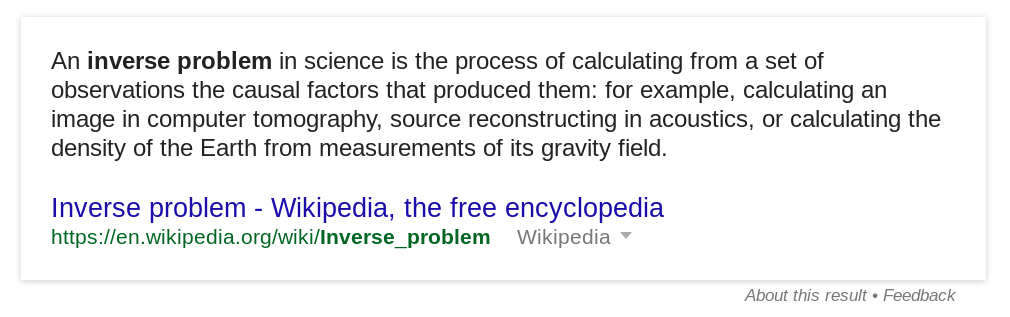
\includegraphics[width=\textwidth]{\basedir/inverse-problem-defn}

        \vspace{2em}
        \only<2->{

        {\large \it cue ominous music }
        }
    \end{center}

\end{frame}

\begin{frame}{}

    {\struct Usually,}
    the {\newthing forwards problem}: 
    \[ \text{ history } \mapsto \text{ what data? } \]
    is easy, but 
    the {\newthing inverse problem}:
    \[ \text{ data } \mapsfrom \text{ what history? } \]
    is {\newthing hard}

    \pause
    \vspace{2em}

    because many possible histories \\
    map to (nearly) the same data.

\end{frame}



%%%%%%%
\begin{frame}{Slow and steady}

    Best-fit model uses only the shape of the range {\struct (flat!)},

    but better fit should be possible.

    \begin{overlayarea}{\textwidth}{0.8\textheight}
        \centering
        \vfill

            % Lake Manix; Mojave River
        % \includegraphics[height=0.8\textheight]{\basedir/glaciallakes.png}
        \includegraphics<2>[height=0.75\textheight]{\basedir/lakemap4.png}
        % \includegraphics<3>[height=0.8\textheight]{\basedir/run_580117_iter_0001_trees-and-things-01}
        % \includegraphics<3>[width=\textwidth]{\basedir/run_580117_iter_0001_trees-and-things-05}

    \end{overlayarea}

\end{frame}


%%%%%%%%% %%%%%%%%%%%% %%%%%%%%%%%%
\section{Next steps}

%%%%%%%%
\begin{frame}{What's next}

  \begin{columns}[c]
    \begin{column}{.6\textwidth}
  Population Viability Analysis: (Jaime Ashander)

  \begin{itemize}

      \item landscape-scale individual-based simulation
      \item inform with the literature
      \item {\newthing but:} juvenile dispersal almost totally unknown
      \item fit to genetic data (divergence, local frequency spectra, haplotypes)

  \end{itemize}
    \end{column}
    \begin{column}{.4\textwidth}
        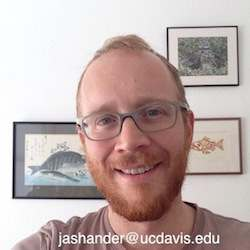
\includegraphics[width=\textwidth]{\basedir/jaime}
    \end{column}
  \end{columns}

\end{frame}


%%%%%%%%%% %%%%%%%%%%%%% %%%%%%%%%%

\begin{frame}{}

  \begin{columns}[c]
    \begin{column}{.4\textwidth}
      \begin{center}
        {\struct Collaborators:}

          {Evan McCartney-Melstad}

          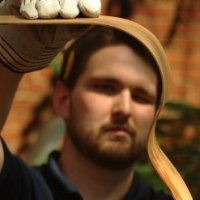
\includegraphics[width=\textwidth]{\basedir/evan}

      {Gideon Bradburd}

          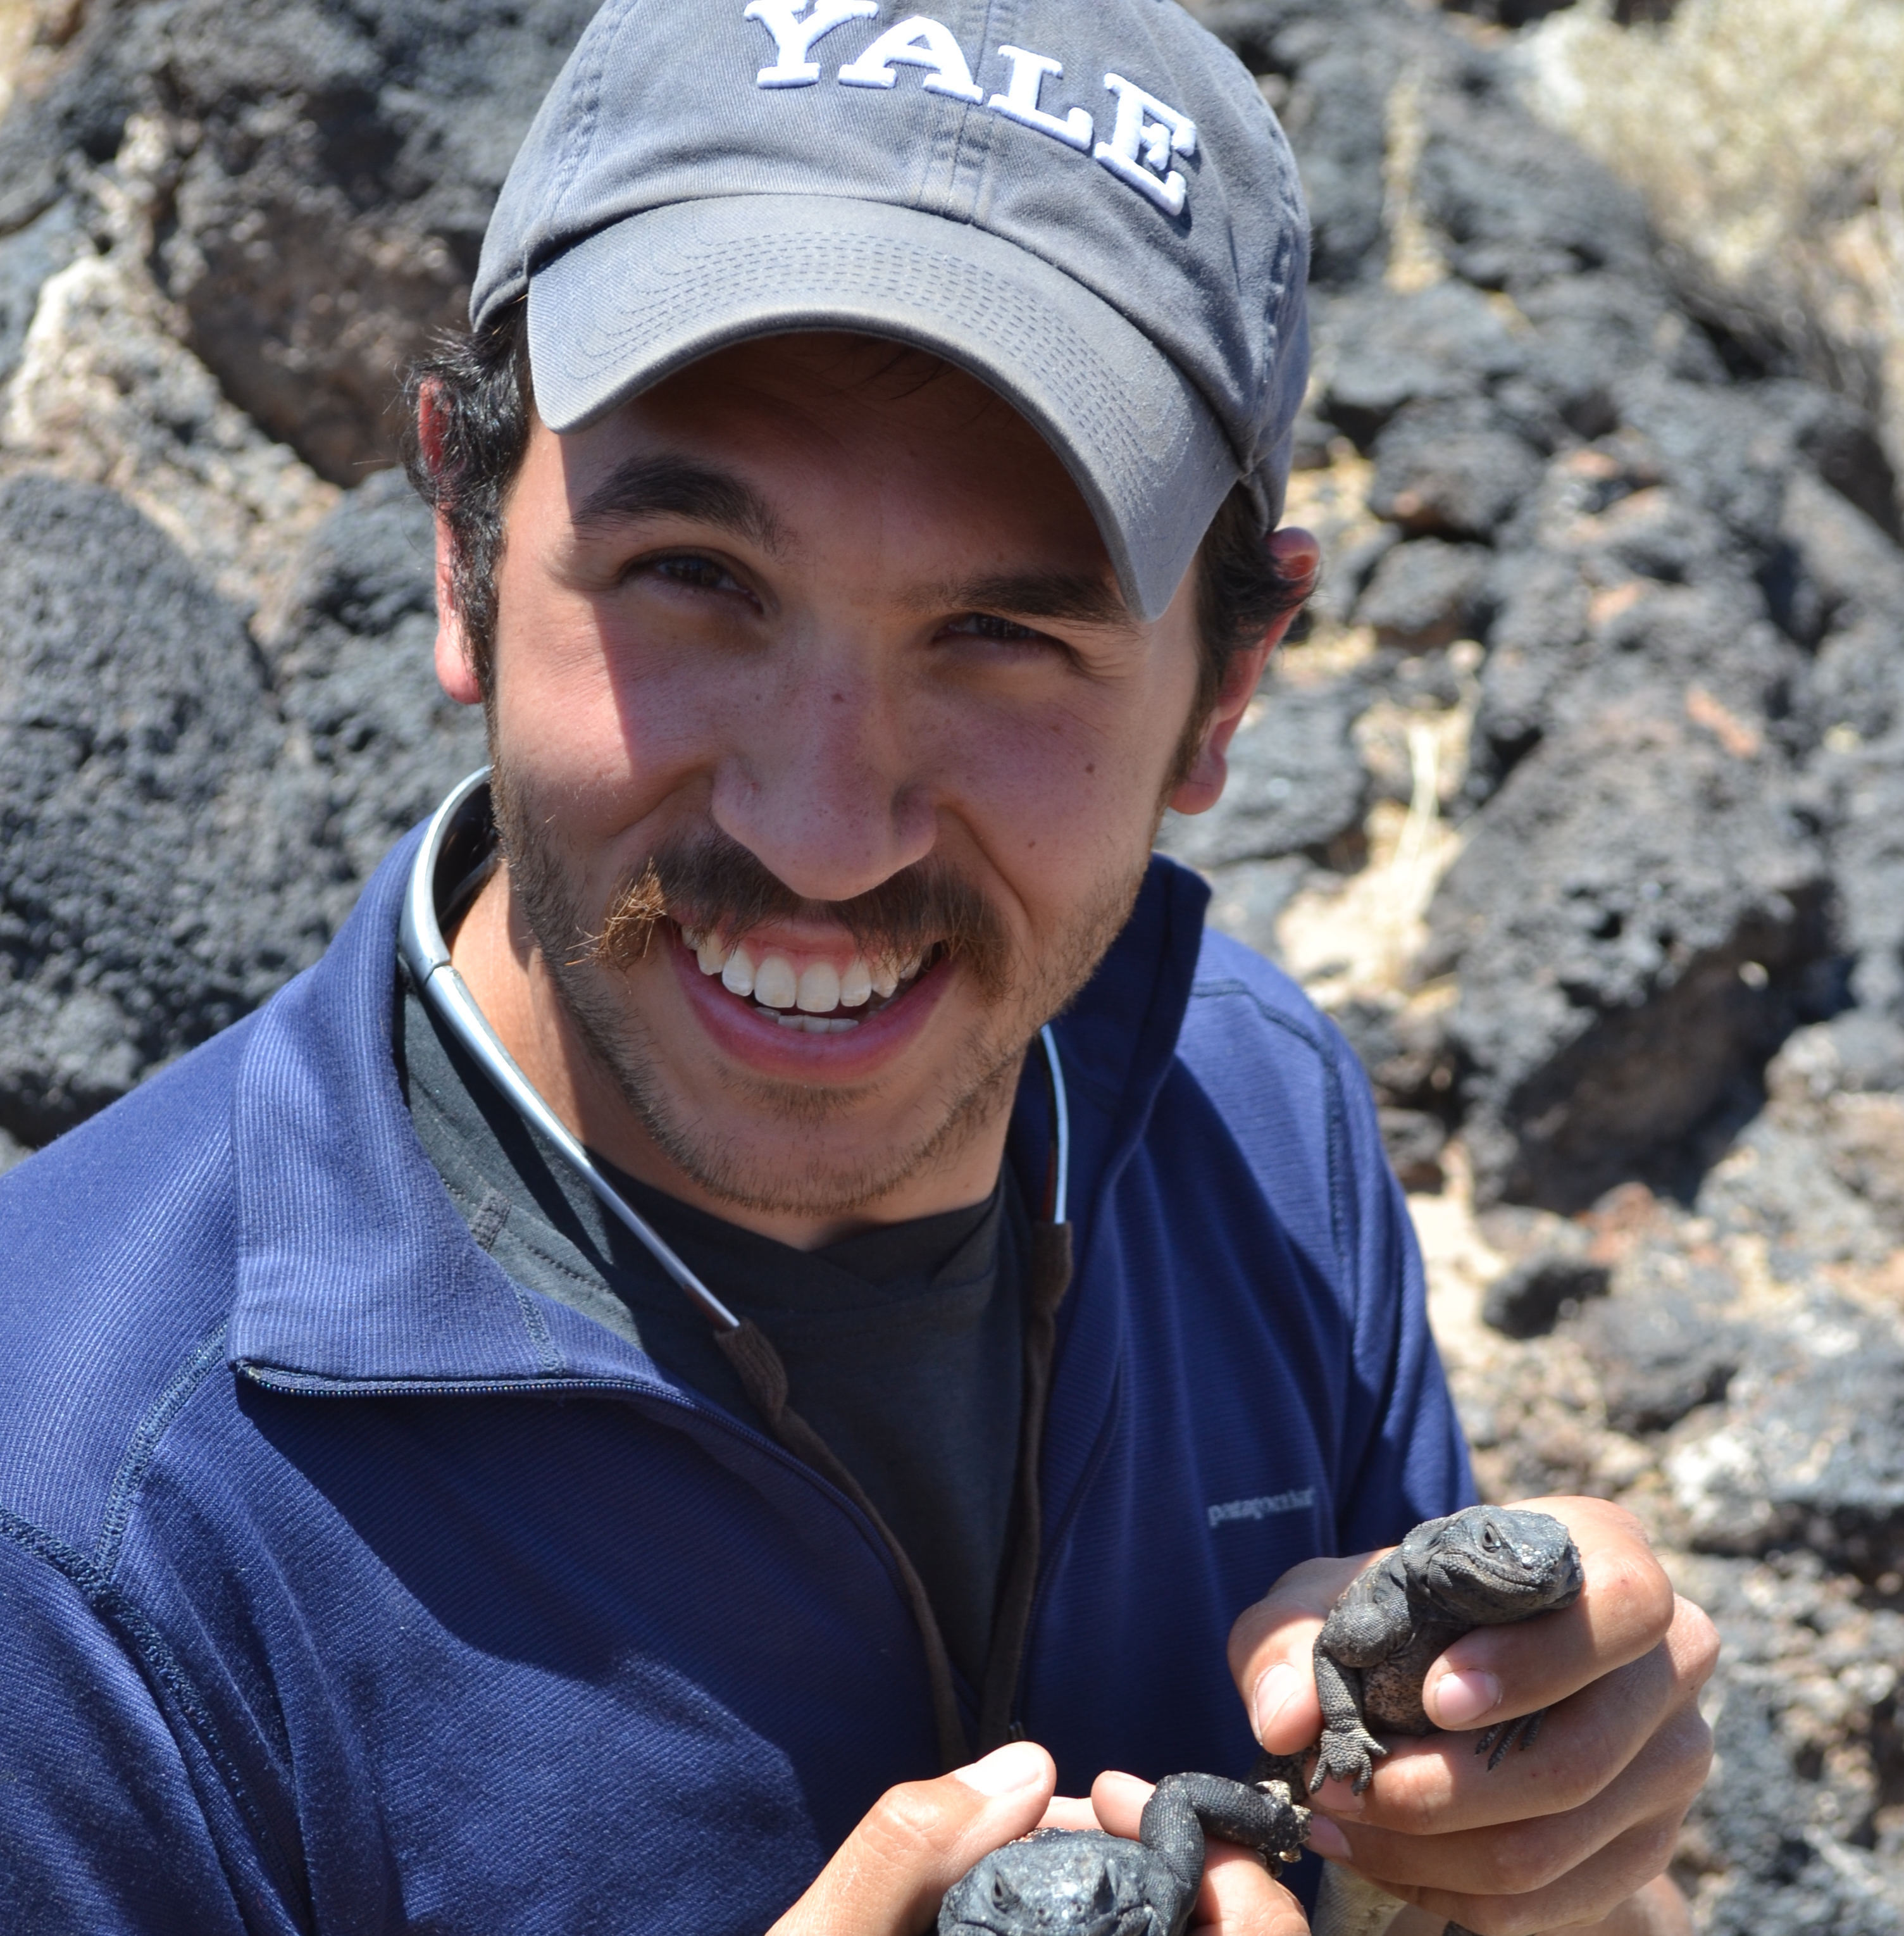
\includegraphics[width=\textwidth]{\basedir/gideon-chuckwallas}

      \end{center}
    \end{column}
    \begin{column}{.6\textwidth}

        \vspace{-2em}
      {Brad Shaffer}

        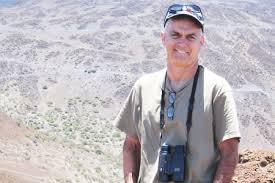
\includegraphics[width=0.75\textwidth]{\basedir/brad}

        Roy Averill-Murray (US F\&WS)

        Erik Lundgren (USC)
      \vspace{0.5em}

        Jannet Vu (UCLA)
      \vspace{0.5em}

      \textbf{Data:}
      Fran Sandmeier, Chava Weitzman, Bridgette Hagerty, Dick Tracy
      \vspace{0.5em}

      \textbf{Funding:}
        CA DFW \textit{and} US F\&WS \\
      NSF: ABI // 
      Sloan Foundation

    \end{column}
  \end{columns}

\end{frame}

\begin{frame}{ }

    \centering
    \vfill

    \Large Thanks!

    \vfill
    {\aside more on tortoises:}\\
    {\it What's in a tortoise nose? Microbial patterns across space.} \\
    Chava Weitzman -- 10am Tue 9AB
    \vfill

\end{frame}
%%%%%%%%%% %%%%%%%%%%%%% %%%%%%%%%%

\section*{More details about fitting hitting times}

%%%%%
\begin{frame}{The rest of the method}
  \begin{columns}
    \begin{column}{0.5\textwidth}
      \begin{itemize}

        \item<1-> Sequence divergence \\
          $\approx$ {\newthing mean hitting times} of a lineage
          \vspace{2em}

        \item<2-> fit parameters by solving PDE 
          % \\ {\aside (multigrid methods)}

        % \item<2-> as are {\newthing derivatives}
        %   with respect to the parameters
           \vspace{2em}

        \item<3-> {\newthing Results:} quantitative comparison of different development scenarios.

      \end{itemize}
    \end{column}
    \begin{column}{0.5\textwidth}
      \centering
      \includegraphics<1>[height=.9\textheight]{\basedir/resistance-approx-right}
      % \only<2>{
      %   \begin{align*}
      %     \rho(x) \nabla \cdot ( u(x) \nabla h_A(x) ) &= -1  \\
      %     \qquad \text{for } x \notin &A  \\
      %     h_A(x) &= 0  \\
      %      \qquad \text{for } x \in &A   
      %   \end{align*}
      % }
      \only<2>{
      \vspace{-.4in}

      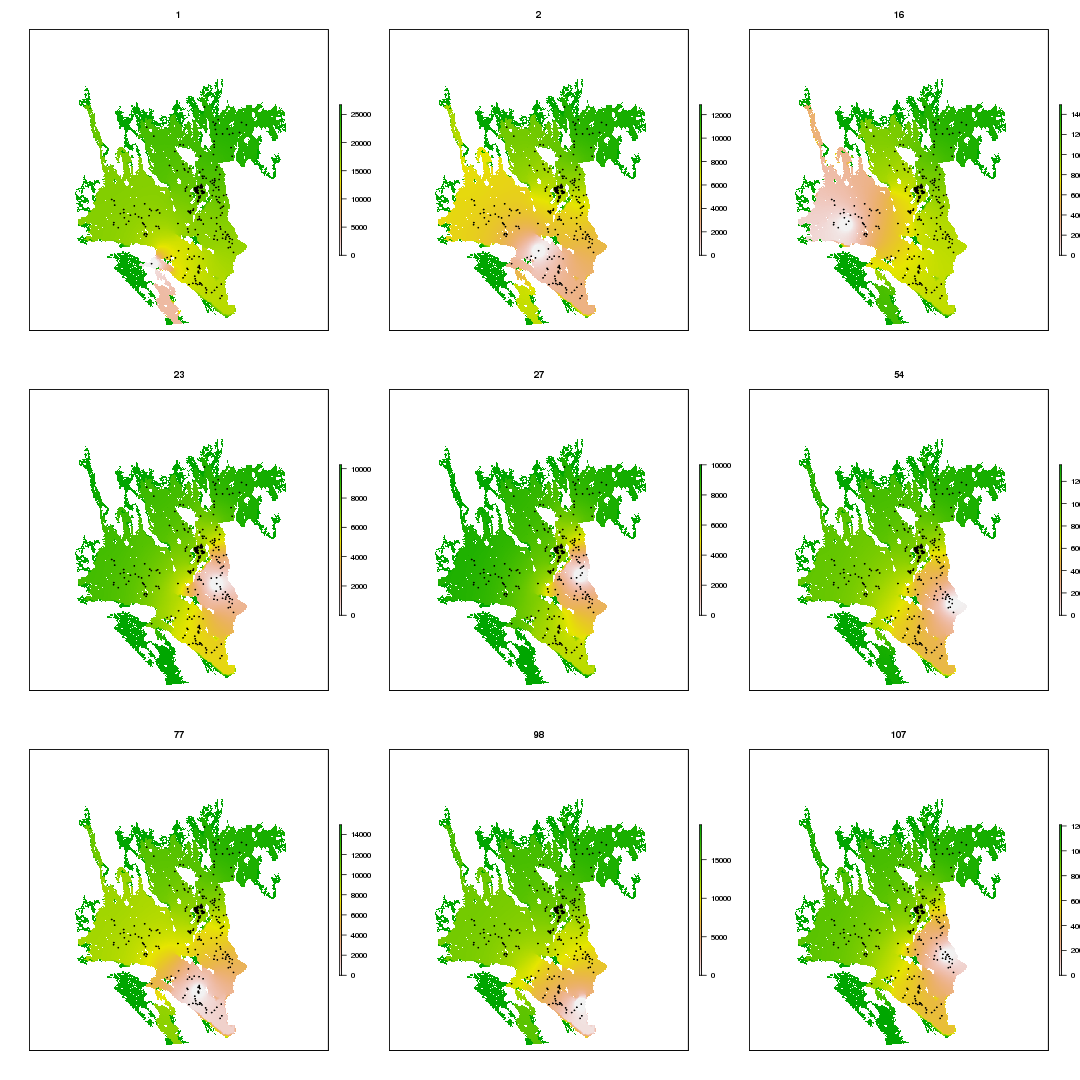
\includegraphics[height=\textheight]{\basedir/example-hitting-times}
      }
      \only<3>{
        % \includegraphics[width=0.8\textwidth]{\basedir/tort-times-alt-1.png}
        % \includegraphics[width=0.8\textwidth]{\basedir/tort-times-alt-2.png}
        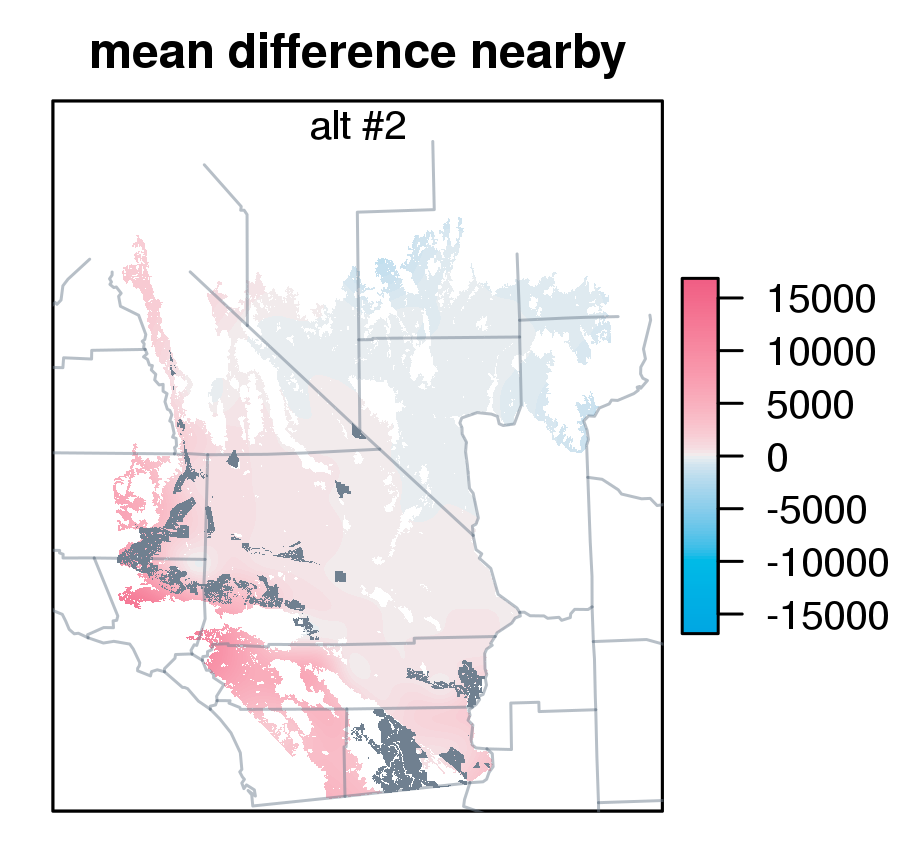
\includegraphics[width=0.8\textwidth]{\basedir/tort-times-alt-2-cropped.png}
      }
    \end{column}
  \end{columns}
\end{frame}



%%%%%
\begin{frame}{Pairwise divergence and hitting times}
      \includegraphics<1>[width=\textwidth]{\basedir/lineages-hitting-time-coal}
      \includegraphics<2>[width=\textwidth]{\basedir/lineages-hitting-time-divergence}
      \includegraphics<3>[width=\textwidth]{\basedir/lineages-hitting-time-divergence-decomp}
      % \includegraphics<4>[width=\textwidth]{\basedir/lineages-hitting-time-divergence-notation}
\end{frame}

%%%%%%%
\begin{frame}{A more tractable problem}
  \begin{center}
      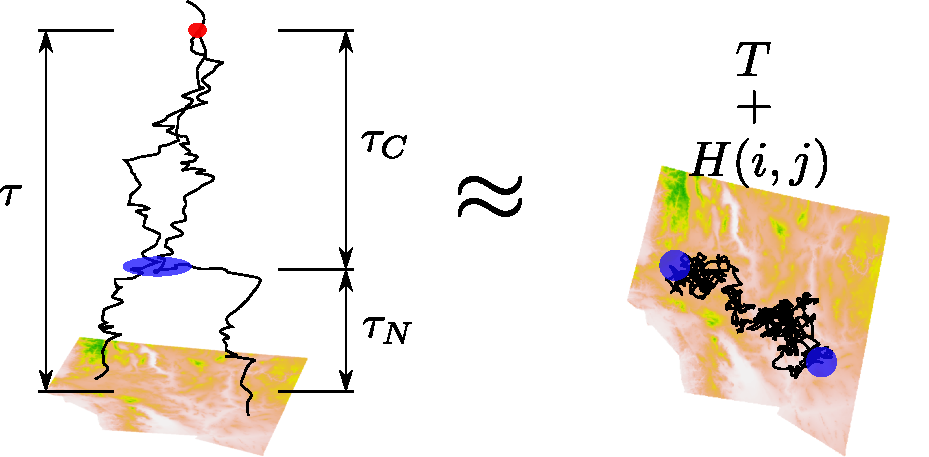
\includegraphics[width=\textwidth]{\basedir/lineages-hitting-time-resistance-coal}
  \end{center}
  Replace {\oldthing $\tau_N$} by commute time \\
  (a.k.a.\ {\newthing resistance distance}, McRae et al)
  \begin{align*}
    N(i,j) &= \E[ \text{( time to get near $j$ started from $i$ )} ] \\
    H(i,j) &\approx \frac{ N(i,j) + N(j,i) }{2} .
  \end{align*}
\end{frame}

%%%%%%%
\begin{frame}{A more tractable problem}
  \begin{center}
      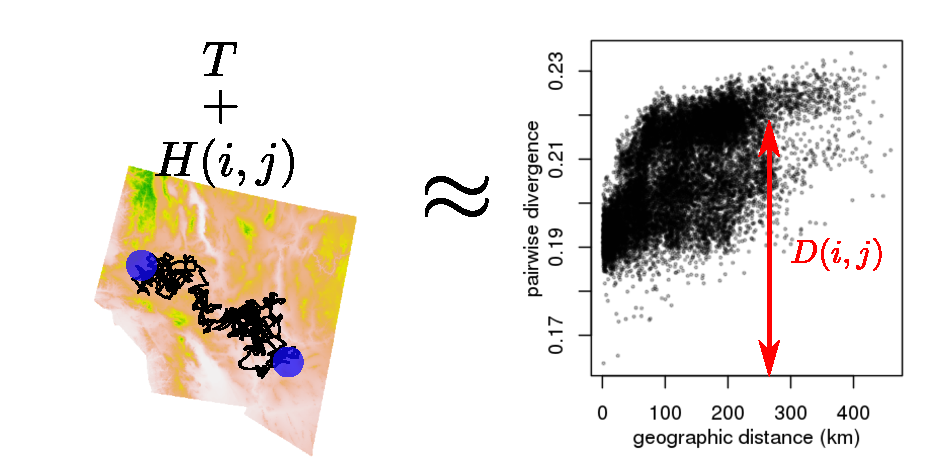
\includegraphics[width=\textwidth]{\basedir/lineages-hitting-time-resistance-divergence}
  \end{center}
  Find parameters $\alpha$, $\beta$, $\gamma$, $T$ to minimize
  \[
  \sum_{ij} | D(i,j) - T - H(i,j) |^2
  \]
\end{frame}

%%%%%%%
\begin{frame}{Fitting hitting times}

  Parameters $\alpha$, $\beta$, $\gamma$ determine $u$ and $\rho$:
  \[
  Gf(x) := \rho(x) \nabla \cdot ( u(x) \nabla f(x) ) .
  \]
  Then
  \[
  h_A(x) := \E[ \text{ time for $X_t$ to hit $A$ from $x$ } ] ,
  \]
  solves
  \begin{align*}
    G h_A(x) &= -1  \qquad \text{for } x \notin A \\
    h_A(x) &= 0  \qquad \text{for } x \in A 
  \end{align*}
  {\struct Keywords:} multigrid methods for elliptic PDE.
  

  \ldots and we can get derivatives by solving the same sort of equation:
  \begin{align*}
    G (\partial_\alpha h_A(x)) &= -(\partial_\alpha G) h_A(x)  \\
    G (\partial_\alpha^2 h_A(x)) &= -(\partial_\alpha^2 G) h_A(x) -2 (\partial_\alpha G)(\partial_\alpha h_A(x))
  \end{align*}
  \ldots and use a \alert{trust region algorithm} to optimize.

\end{frame}

%%%%%
\begin{frame}{}
  \fullslide{
  \centering
  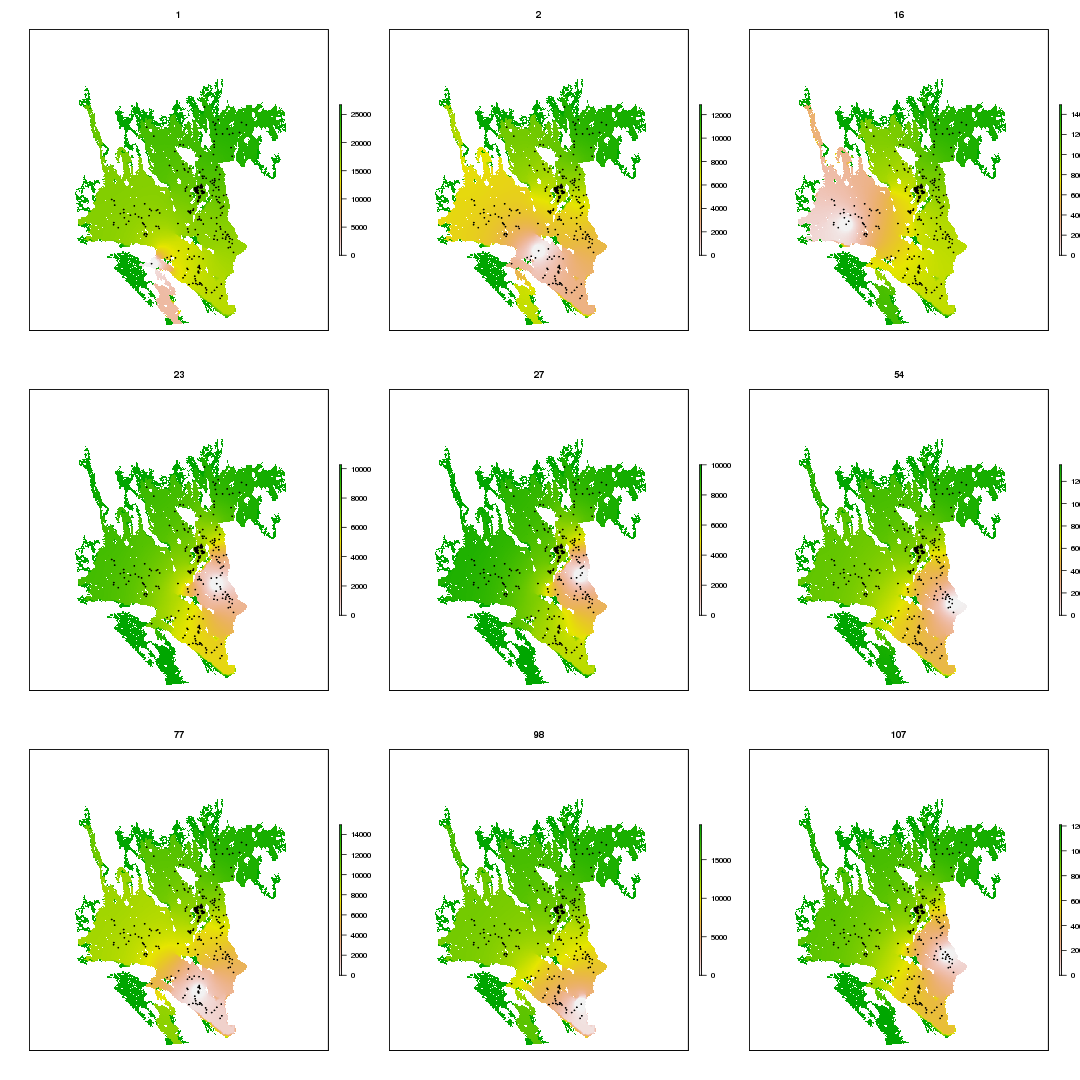
\includegraphics[height=\textheight]{\basedir/example-hitting-times}
  }
\end{frame}


\end{document}
